\subsection{Arquitetura}


%
% Simple topology
%
\begin{frame}\frametitle{Arquitetura Openflow}

    \begin{itemize}
    \item Uma topologia simples:
    \end{itemize}
    
	\begin{figure}[h]
        \centering
        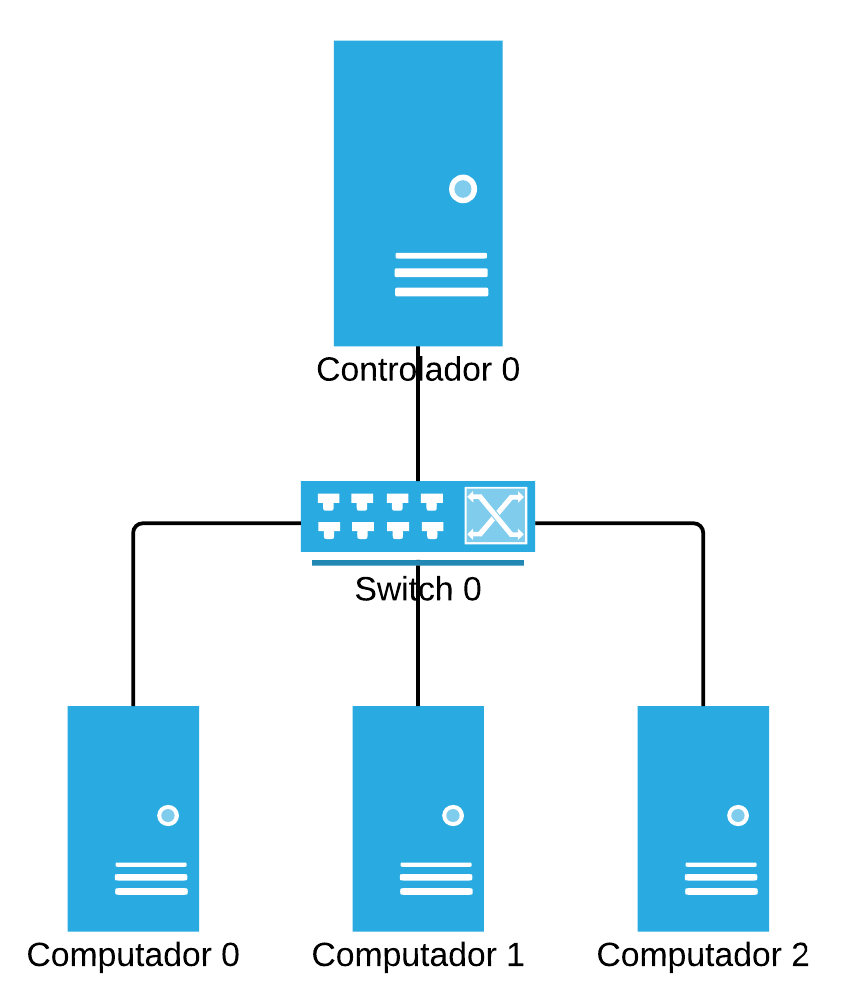
\includegraphics[scale=0.3]{images/simple-topology.png}
    \end{figure}
\end{frame}


%
% N openflow 
%
\begin{frame}\frametitle{Arquitetura Openflow}

    \begin{itemize}
    \item Um controlador para vários \emph{Switches}
    \end{itemize}
    
	\begin{figure}[h]
        \centering
        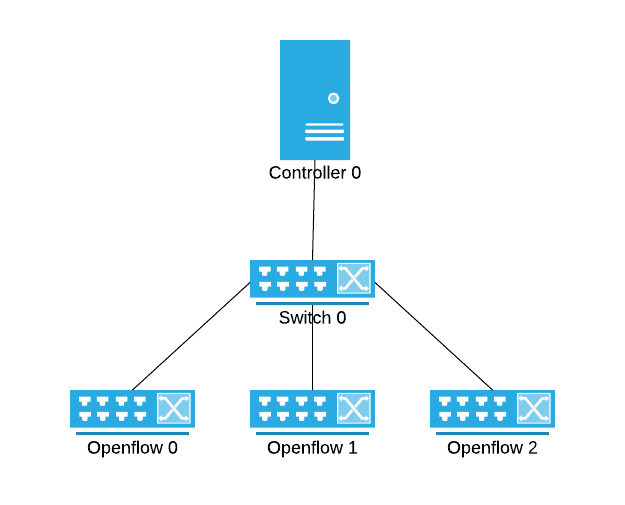
\includegraphics[scale=0.4]{images/n-openflow-switches.png}
    \end{figure}
\end{frame}


%
% SDN inter domain
%
\begin{frame}\frametitle{Arquitetura Openflow}

    \begin{itemize}
    \item Comunicação entre domínios de rede
    \end{itemize}
    
   
	\begin{figure}[h]\hspace*{-1cm}
        \centering
        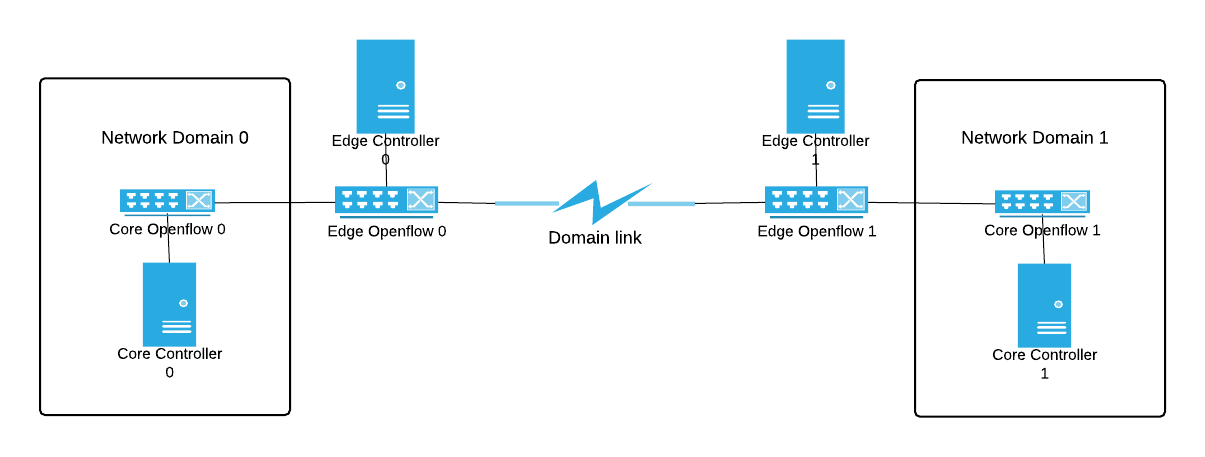
\includegraphics[scale=0.3]{images/edge-core-sdn.png}
    \end{figure}
\end{frame}



%
% Distributed openflow controller
%
\begin{frame}\frametitle{Arquitetura Openflow}

    \begin{itemize}
    \item Controlador distribuído
    \end{itemize}
    
	\begin{figure}[h]
        \centering
        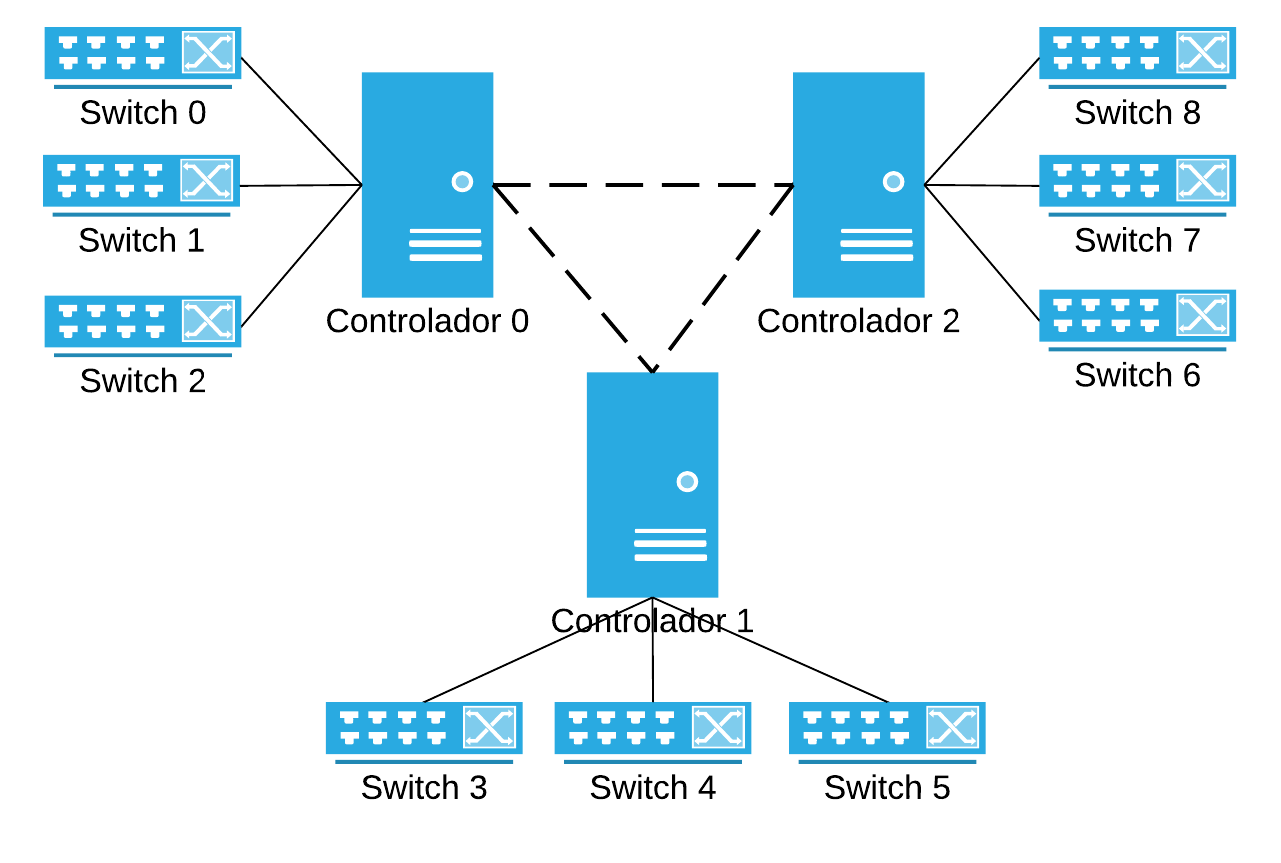
\includegraphics[scale=0.4]{images/distributed_sdn_controller.png}
    \end{figure}
\end{frame}
